
\chapter{遗忘理论的定义及其语义属性}\label{chapter03}
{\em 本章首先通过扩展互模拟的概念,给出$\CTL$下遗忘理论的定义。其次,探索遗忘理论的一般通用属性,这些属性包括:模块化(Modularity)性质、交换性(Commutativity)、齐次性(Commutativity)等属性。}

\section{引言}
从一个公式中“遗忘”掉一些原子命题得到的结果应该不违背定义在剩余原子命题集合上的公式,也就是说对于剩余原子命题集合上的公式,原始公式能够逻辑蕴涵它当且仅当遗忘得到的结果能过逻辑蕴涵它。从模型的角度来讲,遗忘得到的结果的模型与原始公式的模型在除去被遗忘的那些原子命题之后是能够想互模拟的。\emph{互模拟}描述的是两个在行为上能够相互替代的转换系统\cite{Baier:PMC:2008}。在本文中,转换系统被描述成为Kripke结构。因此为了描述遗忘理论,这部分给出在给定原子命题集合上的Kripke结构(或$\Ind$-结构)上的互模拟的定义及其性质。

基于互模拟的概念,给出了$\CTL$下遗忘理论的定义。与后面章节将要讲述的约束$\CTL$下的遗忘相对应,这部分探索没有约束的遗忘理论的一般属性。

\section{$V$-互模拟}

这部分给出定义在给定原子命题集合$V$上的互模拟的概念,本文称之为$V$-互模拟。尽管在文章~\cite{Yan:AIJ:2009}中给出了相似的概念,但是如在基础知识部分所述,$S5$的语义是定义在一种特殊的Kripke结构($\MPK$-解释)下的,因而不具有一般性。接下来探讨一种更加一般的$V$-互模拟。


\begin{definition}[$V$-互模拟]
	\label{def:VInd:bisimulation}
	给定原子命题集合$V\subseteq\cal A$、索引集合$I\subseteq \Ind$和初始$\Ind$-结构 $\Hm_i=(S_i, R_i,L_i, [\_]_i, s_0^i)~(i=1,2)$。
	对关系 $\Hb_V \subseteq S_1 \times S_2$和任意的$s_1 \in S_1$和$s_2 \in S_2$,若$(s_1, s_2)\in \Hb_V$蕴涵下列条件,则称 $\Hb_V$ 是 $\Hm_1$ 和 $\Hm_2$之间的一个 $V$-互模拟关系:
	\begin{itemize}
		\item[(i)] $L_1(s_1) - V = L_2(s_2) -V$;
		\item[(ii)] $\forall r_1\in S_1$, 若$(s_1, r_1)\in R_1$,则$\exists r_2 \in S_2$ 使得 $(s_2,r_2) \in R_2$ 和 $(r_1, r_2) \in \Hb_V$;
		\item[(iii)] $\forall r_2\in S_2$,若$(s_2, r_2)\in R_2$,则 $\exists r_1 \in S_1$ 使得 $(s_1,r_1) \in R_1$ 和 $(r_1, r_2)\in \Hb_V$。
	\end{itemize}
\end{definition}


若$\Hm_1$ 和 $\Hm_2$之间存在一个 $V$-互模拟关系$\Hb_V$使得$(s_1, s_2)\in \Hb_V$,则称两个 $\Ind$-结构 ${\cal K}_1 = (\Hm_1, s_1)$ 和 ${\cal K}_2 = (\Hm_2, s_2)$ 是 $V$-{\em 互模拟},记为${\cal K}_1 \lrto_V {\cal K}_2$。
令$i\in \{1,2\}$,$\pi_i=(s_{i,1},s_{i,2},\ldots)$为$\Hm_i$上的路径,若对任意的$j \ge 1$都有$ {\cal K}_{1,j} \lrto_V {\cal K}_{2,j}$,则称这两条路径是$V$-{\em 互模拟}的,记为$\pi_1 \lrto_V \pi_2$,其中${\cal K}_{i,j}=(\Hm_i,s_{i,j})$。


直观地说,若两个状态在不考虑$V\subseteq\cal A$中的元素时,其行为是相同的,则称这两个状态是“互模拟”的。
当 $V=\emptyset$,$V$-互模拟的三个条件即为$\CTL$中的互模拟要满足的条件。
下文中当初始$\Ind$-结构能从上写文中清楚地知道时,简写 ${\cal K}_1 \lrto_V {\cal K}_2$ 为 $s_1 \lrto_V s_2$。

%为此,首先给出能够描述一定深度$n\in \mathbb{N}$的计算树之间的$V$-互模拟关系,记为$\Hb_n^V$。令$V\subseteq \Ha$是原子命题的集合,$i\in \{1,2\}$,$\Hm_i=(S_i,R_i,L_i,s_0^i)$(或$\Hm_i=(S_i,R_i,L_i,[\_]_i,s_0^i)$)是初始结构($\Ind$-Kripke结构),${\cal K}_i=(\Hm_i, s_i)$是$\MPK$-结构(或$\Ind$-结构)。$\Hb_n^V$被递归定义如下:
%\begin{itemize}
%	\item 若$L_1(s_1)-V=L_2(s_2)$,则$({\cal K}_1,{\cal K}_2) \in \Hb_0^V$;
%	\item 对任意$n\ge 0$,若满足下面几个条件,则$({\cal K}_1,{\cal K}_2)\in \Hb_{n+1}^V$成立:
%		\begin{itemize}
%			\item $({\cal K}_1,{\cal K}_2) \in \Hb_0^V$;
%			\item 对任意$(s_1,s_1')\in R_1$,存在$(s_2,s_2')\in R_2$使得$({\cal K}_1',{\cal K}_2') \in \Hb_n^V$;
%			\item 对任意$(s_2,s_2')\in R_2$,存在$(s_1,s_1')\in R_1$使得$({\cal K}_1',{\cal K}_2') \in \Hb_n^V$。
%		\end{itemize}
%\end{itemize}
%其中${\cal K}_i'=(\Hm_i,s_i')$。
%
%当所谈及的原子命题的集合$V$很显然的时候,上述$\Hb_n^V$中的$V$可以省略,记为$\Hb_n$。此外,当讨论的$\Hm_i$$(i=1,2)$是显然的时候,可以使用$(s_1,s_2) \in \Hb_n$代替$((\Hm_1,s_1),(\Hm_2,s_2)) \in \Hb_n$。
%此时,$V$-互模拟关系就可以定义如下:
%\begin{definition}[$V$-互模拟]\label{def:V-bisimulation}
%	令$V$是$\Ha$的一个子集,$i\in \{1,2\}$, ${\cal K}_1$和${\cal K}_2$是$\MPK$-结构(或$\Ind$-结构)。
%	\begin{itemize}
%		\item ${\cal K}_1$和${\cal K}_2$是$V$-互模拟的,当且仅当对所有的$n \ge 0$都有$({\cal K}_1, {\cal K}_2)\in \Hb_n$。若${\cal K}_1$和${\cal K}_2$是$V$-互模拟的,则记为${\cal K}_1 \lrto_V {\cal K}_2$。
%		\item 对$\Hm_i$上的路径$\pi_i=(s_{i,1},s_{i,2},\dots)$,若对于任意的$j\in \mathbb{N}_{\ge 1}$\footnote{$\mathbb{N}_{\ge 1}$是大于等于1的整数的集合。}都有${\cal K}_{1,j} \lrto {\cal K}_{2,j}$,则$\pi_1 \lrto_V \pi_2$。其中${\cal K}_{i, j}=(\Hm_i, s_{i,j})$。
%	\end{itemize}
%\end{definition}
%
%上述$V$-互模拟的定义是现有互模拟定义的一般化,这可以从下面几个方面来体现\footnote{在其他领域也有类似的定义,如:定义在数据库相关文献中的概念$k$-互模拟\cite{kaushik2002updates}。$k$-互模拟概念中涉及与本文$\Hb_n$类似的定义,只是其关系是从相反的方向(即:从孩子到父节点的方向)来说明的。此外,值得一提的是,本文的$V$-互模拟的概念是定义在$\MPK$-结构上的。}。
%首先,当给定的$V$为空集且谈论指定的初始状态时,本文的$V$-互模拟与定义在Baier等文章里的互模拟等价(定义7.1\cite{Baier:PMC:2008})的概念一致。
%其次,在同一文章里的基于状态的互模拟(定义7.7\cite{Baier:PMC:2008})是定义在给定结构的状态上的,因此与本文的$V$-互模拟(定义在结构的集合上)也不同。
%最后,本文的$\Hb_n$的定义与Browne的论文中的状态等价$E_n$类似,只是后者是定义在状态上\cite{browne1988characterizing}而本文的定义在$\MPK$-结构(或$\Ind$-结构)上。


下面例子呈现结构之间的$V$-互模拟。
\begin{example}\label{exam:vB}
	令${\cal K}_1$,${\cal K}_2$和${\cal K}_3$为三个$\MPK$-结构,其图表示分别如图中的${\cal K}_1$,${\cal K}_2$和${\cal K}_3$所示。它们之间的互模拟关系也如图中标记所示,即${\cal K}_1 \lrto_{\{sp\}} {\cal K}_2$,${\cal K}_2 \lrto_{\{se\}} {\cal K}_3$和${\cal K}_1 \lrto_{\{sp,se\}} {\cal K}_3$。此外,可以看出${\cal K}_1$,${\cal K}_2$和${\cal K}_3$之间是互不互模拟\cite{Baier:PMC:2008}的,即不$\emptyset$-互模拟。
	\begin{figure*}[!htb]
		\centering
		% Requires \usepackage{graphicx}
		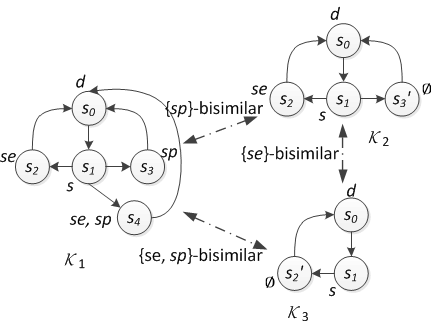
\includegraphics[width=8cm]{chapter03/NVBnewCar.png}\\
		\caption{$\MPK$-结构之间的$V$-互模拟关系}
		\label{Fig:chapter05:v1uv2}
	\end{figure*}
\end{example}

 
 
 $V$-互模拟给出了两个结构之间相互模仿的行为关系,下面的命题给出了这种关系一些关键的性质。
 \begin{proposition}\label{prop:bisimilar:V}
 	令$i$是属于集合$\{1,2\}$的变量,$V_1$和$V_2$是$\Ha$的子集,$s_1'$和$s_2'$是两个状态,$\pi_1'$和$\pi_2'$是两条路径,${\cal K}_j=(\Hm_j,s_j)$$(j=1,2,3)$是$\MPK$-结构(或$\Ind$-结构)。如果$({\cal K}_1 \lrto_{V_1} {\cal K}_2)$且$({\cal K}_2 \lrto_{V_2} {\cal K}_3)$,则:
 	\begin{itemize}
 		\item[(i)] ${\cal K}_1\lrto_{V_1\cup V_2}{\cal K}_3$;
 		\item[(ii)] 若 $V_1 \subseteq V_2$ 则 ${\cal K}_1 \lrto_{V_2} {\cal K}_2$;
 		\item[(iii)] $s_1'\lrto_{V_i}s_2'~(i=1,2)$ 蕴涵$s_1'\lrto_{V_1\cup V_2}s_2'$;
 		\item[(iv)] $\pi_1'\lrto_{V_i}\pi_2'~(i=1,2)$ 蕴涵 $\pi_1'\lrto_{V_1\cup V_2}\pi_2'$;
 		\item[(v)] 对$\Hm_1$上的每条路径 $\pi_{s_1}$,存在$\Hm_2$上的一条路径 $\pi_{s_2}$ 使得 $\pi_{s_1} \lrto_{V_1} \pi_{s_2}$,反之也成立。
 	\end{itemize}
 \end{proposition}
\begin{proof}
	%We prove the cases of $\MPK$-structures, and the cases of $\Ind$-structures are trivial.
	(i) 令 ${\cal M}_j=(S_j,R_j,L_j,[\_]_j,s_0^j)~(j=1,2,3)$,$\Hb$为$s_1$和$s_2$之间的$V_1$-互模拟关系,即 $s_1 \lrto_{V_1} s_2$通过$\Hb$形成$V_1$-互模拟关系,$s_2 \lrto_{V_2} s_3$通过$\Hb''$形成$V_2$-互模拟关系。 令 $\Hb' = \{(w_1, w_3)\mid (w_1, w_2)\in \Hb$ 和 $(w_2, w_3)\in \Hb''\}$。为了证明 ${\cal K}_1\lrto_{V_1\cup V_2}{\cal K}_3$,这里证明$\Hb'$ 是一个 包含$(s_1, s_3)$的$V_1 \cup V_2$-互模拟关系。由于$(s_1,s_2)\in \Hb$ 和 $(s_2, s_3)\in \Hb''$,所以$(s_1, s_3) \in \Hb'$。
	% 		from the (a), (b) and (c) of the previous step (iii) of $X$-bisimulation (where $X$ is a set of atoms).
	对于所有 $(w_1, w_3) \in \Hb'$:
	\begin{itemize}
		\item[(a)] 存在一个 $w_2 \in S_2$使得 $(w_1,w_2)\in \Hb$ 和 $(w_2, w_3)\in \Hb''$,因此由 $w_1 \lrto_{V_1} w_2$可知, $L_1(w_1)-V_1 = L_2(w_2) - V_1$,且由$w_2 \lrto_{V_2} w_3$可知 $L_2(w_2) - V_2 = L_3(w_3) - V_2$。
		%			for all $q \notin V_1$, $q \in L_1(w_1)$ iff $q \in L_2(w_2)$ by $w_1 \lrto_{V_1} w_2$ and for all $q' \notin V_2$, $q'\in L_2(w_2)$ iff $q'\in L_3(w_3)$ by $w_2 \lrto_{V_2} w_3$. 
		所以有 $L_1(w_1) - (V_1 \cup V_2) = L_3(w_3) - (V_1 \cup V_2)$.
		% for all $r\notin V_1 \cup V_2$, $r \in L_1(w_1)$ iff $r \in L_3(w_3)$.
		\item[(b)] $\forall u_1\in S_1$,若 $(w_1, u_1) \in R_1$,则 $\exists u_2\in S_2$ 使得$(w_2, u_2) \in R_2$ 和 $(u_1,u_2)\in \Hb$ (由 $\Hb'$的定义可知$(w_1,w_2)\in \Hb$ 和 $(w_2, w_3) \in \Hb''$); 因而 $\exists u_3 \in S_3$ 使得$(w_3, u_3) \in R_3$ 和 $(u_2, u_3) \in \Hb''$,所以由 $\Hb'$的定义可知 $(u_1, u_3) \in \Hb'$。
		\item[(c)] $\forall u_3\in S_3$,若 $(w_3, u_3) \in R_3$,则 $\exists u_2\in S_2$ 使得 $(w_2, u_2) \in R_2$ 和 $(u_2, u_3) \in \Hb_2$;因此 $\exists u_1 \in S_1$ 使得  $(w_1, u_1) \in R_1$ 和 $(u_1, u_2) \in \Hb$,所以由 $\Hb'$的定义可知$(u_1, u_3) \in \Hb'$。
	\end{itemize}
	
	(ii) 假定 $\Hb_{V_1}$是$\Hm_1$ 和 $\Hm_2$之间的一个 $V_1$-互模拟关系,且 $(s_1, s_2)\in \Hb_{V_1}$。这里证明 $\Hb_{V_1}$ 也是$\Hm_1$ 和 $\Hm_2$之间的一个 $V_2$-互模拟关系。
	对任意的 $(w_1, w_2) \in \Hb_{V_1}$,有:
	\begin{itemize}
		\item 因为$L_1(w_1) - V_1 = L_2(w_2) -V_1$ 和 $V_1 \subseteq V_2$,所以 $L_1(w_1) - V_2 = L_2(w_2) -V_2$;
		\item $\forall r_1 \in S_1$,若 $(w_1,r_1) \in R_1$,因为$\Hb_{V_1}$是$\Hm_1$ 和 $\Hm_2$之间的一个 $V_1$-互模拟关系, 则 $\exists r_2\in S_2$ 使得 $(w_2,r_2)\in R_2$ 和 $(r_1,r_2) \in \Hb_{V_1}$;和
		\item $\forall r_2 \in S_2$,若 $(w_2,r_2) \in R_2$,因为$\Hb_{V_1}$是$\Hm_1$ 和 $\Hm_2$之间的一个 $V_1$-互模拟关系,则 $\exists r_1\in S_1$使得 $(w_1,r_1)\in R_1$ 和 $(r_1,r_2) \in \Hb_{V_1}$。
	\end{itemize}
	
	由于$V_i \subseteq (V_1 \cup V_2)$( $i = 1, 2$),则(iii) 是 (ii)的一种特殊情况 due to $V_i \subseteq (V_1 \cup V_2)$,因而(iv) 从(iii)可以容易得到。
	
	(v) 可以从$V$-互模拟的定义容易得到,因为$s_1 \lrto_{V_1} s_2$ (即:${\cal K}_1\lrto_{V_1}{\cal K}_2$)。	
\end{proof}

 
 在命题~\ref{pro:div}中,性质(iii)-(v)是$V$-互模拟的标准属性,含义比较直观。性质(i)表示如果一个结构分别与另外的两个结构具有$V_1$和$V_2$-互模拟关系,则这两个结构是$V_1\cup V_2$-互模拟的(如图~\ref{Fig:chapter05:v1uv2}所示)。如后文所示,这一性质对遗忘理论性质的探索至关重要。性质(ii)表示若两个结构是$V_1$-互模拟的,则对于任意的$V_2$,若$V_1 \subseteq V_2$则这两个结构是$V_2$-互模拟的。
 
 从互模拟的定义上来看,如果两个结构是$V$-互模拟的,那么对于与$V$中的原子命题无关的公式$\varphi$来说,这两个结构同时满足或不满足$\varphi$。这一性质可以形式化地描述如下:
 
 \begin{theorem}\label{thm:V-bisimulation:EQ}
 	令$V\subseteq \Ha$是原子命题的集合,${\cal K}_i$ $(i=1,2)$是两个具有$V$-互模拟的$\MPK$-结构,即:${\cal K}_1 \lrto_V {\cal K}_2$,$\Phi$是一个$\CTL$公式且$\IR(\Phi, V)$。则有${\cal K}_1\models \Phi$当且仅当${\cal K}_2\models \Phi$。
 \end{theorem}
\begin{proof}
	这一结论可以从$\CTL$公式的结构归纳地来证明。此外,不失一般性地可以假设$\Var(\Phi) \cap V=\emptyset$,${\cal K}_1=(\Hm,s)$和${\cal K}_1=(\Hm',s')$。
	
	情形1:$\Phi = p$ ($p\in \Ha -V$).
	
	$(\Hm,s)\models \Phi$当且仅当$p\in L(s)$ \hfill (可满足关系的定义)\\
	$\LRto$ $p\in L'(s')$ \hfill ($s \lrto_v s'$)\\
	$\LRto$ $(\Hm',s') \models \Phi$。
	
	情形2:$\Phi = \neg \psi$.
	
	$(\Hm,s)\models \Phi$当且仅当$(\Hm,s) \not \models \psi$\\
	$\LRto$ $(\Hm',s')\not \models \psi$  \hfill (归纳假设)\\
	$\LRto$ $(\Hm',s') \models \Phi$。
	
	情形3:$\Phi = \psi_1 \vee \psi_2$.
	
	$(\Hm,s)\models \Phi$\\
	$\LRto$ $(\Hm,s) \models \psi_1$或$(\Hm,s) \models \psi_2$\\
	$\LRto$ $(\Hm',s')  \models \psi_1$或$(\Hm',s') \models \psi_2$ \hfill (归纳假设)\\
	$\LRto$ $(\Hm',s') \models \Phi$。
	
	情形4:$\Phi=\EXIST\NEXT\psi$.
	
	$(\Hm,s)\models \Phi$\\
	$\LRto$ 存在一条路径$\pi=(s,s_1,\dots)$使得$(\Hm,s_1)\models \psi$\\
	$\LRto$ 存在一条路径$\pi'=(s',s_1',\dots)$使得$\pi \lrto_V \pi'$ \hfill ($s \lrto_V s'$,Proposition~\ref{pro:div})\\
	$\LRto$ $s_1 \lrto_V s_1'$ \hfill ($\pi \lrto_V \pi'$)\\
	$\LRto$ $(\Hm',s_1') \models \psi$   \hfill   (归纳假设)\\
	$\LRto$ $(\Hm',s')\models \Phi$。
	
	情形5:$\Phi = \EXIST \GLOBAL \psi$.
	
		$(\Hm,s)\models \Phi$\\
	$\LRto$ 存在一条路径$\pi=(s=s_0,s_1,\dots)$使得对于任意的$i\ge 0$都有$(\Hm,s_i)\models \psi$\\
	$\LRto$ 存在一条路径$\pi'=(s'=s_0',s_1',\dots)$使得$\pi \lrto_V \pi'$ \hfill ($s \lrto_V s'$,Proposition~\ref{pro:div})\\
	$\LRto$ 对于任意的$i\ge 0$都有$s_i \lrto_V s_i'$ \hfill ($\pi \lrto_V \pi'$)\\
	$\LRto$ 对于任意的$i\ge 0$都有$(\Hm,s_i') \models \psi$ \hfill (归纳假设)\\
	$\LRto$ $(\Hm',s')\models \Phi$。
	
	情形6:$\Phi = \EXIST (\psi_1 \UNTILL \psi_2)$.
	
	$(\Hm,s) \models \Phi$\\
	$\LRto$ 存在一条路径$\pi=(s=s_0,s_1,\dots)$和$i \ge 0$使得$(\Hm,s_i) \models \psi_2$,且对所有的$0\leq j <i$都有$(\Hm,s_j)\models \psi_1$\\
	$\LRto$ 存在一条路径$\pi'=(s'=s_0',s_1',\dots)$使得$\pi \lrto_V \pi'$ \hfill ($s \lrto_V s'$,Proposition~\ref{pro:div})\\
	$\LRto$ $(\Hm',s_i') \models \psi_2$,且对于所有的$0\leq j <i$都有$(\Hm',s_j')\models \psi_1$  \hfill  (归纳假设)\\
	$\LRto$ $(\Hm',s')\models \Phi$。
\end{proof}

值得注意的上,上述定理中个公式 $\phi$ 必须不包含索引。否则, ${\cal I}$-结构 中的索引函数可能会影响公式可满足性。
例:令 $\phi=\EXIST_{\tuple{1}}\NEXT p$、
${\cal K}=(\Hm,s)$ 和 $\Hm=(S,R,L,[\_],s_0)$,其中 $S=\{s_0,s_1\}$, $L(s_0)=\emptyset$、 $L(s_1)=\{p\}$、
$R=\{(s_0,s_1),(s_0,s_0),(s_1,s_1), (s_1,s_0)\}$ 和 $[1]=\{(s_0,s_1), (s_1,s_1)\}$。容易检查${\cal K}\models\phi$。
令 ${\cal K}'=(\Hm',s)$ 和 $\Hm'=(S,R,L,[\_]',s_0)$,其中 $[1]'=\{(s_0,s_0),(s_1,s_1)\}$。
显然 ${\cal K}\lrto_{\{q\}}{\cal K}'$, $\IR(\phi,\{q\})$。但是,${\cal K}'\not\models\phi$。

\begin{example}
	令$\varphi_1 = d \wedge \EXIST\FUTURE se \wedge \ALL\GLOBAL(se \rto \ALL\NEXT d)$和$\varphi_2=d \wedge \ALL\NEXT se$是两个$\CTL$公式,且$\IR(\varphi_1,\{sp\})$ 和 $\IR(\varphi_2,\{sp\})$成立。因此可以验证图~\ref{Fig:chapter05:v1uv2}中的${\cal K}_1$和${\cal K}_2$都满足$\varphi_1$,但是都不满足$\varphi_2$。
\end{example}

\begin{definition}[互模拟等价(bisimilar equivalence)]\label{def:bisimular:equivalene}
	给定原子命题的集合$V\subseteq {\cal A}$,公式$\varphi$ 和 $\psi$。若对任意的 ${\cal K}\models \varphi$都存在一个${\cal K}'\models\psi$使得${\cal K}\lrto_V{\cal K}'$,且对任意的${\cal K}'\models\psi$都存在一个${\cal K}\models \varphi$使得${\cal K}\lrto_V{\cal K}'$,则称公式$\varphi$ 和 $\psi$ 是 {\em $V$-互模拟等价的(bisimilar equivalence)},记为 $\varphi\equiv_V\psi$。
\end{definition}

由定义~\ref{def:VInd:bisimulation} 和 \ref{def:bisimular:equivalene},和命题~\ref{prop:bisimilar:V}可容易得出下列引理。
\begin{lemma}~\label{lem:eqR}
	对任意的$V\subseteq\cal A$,  $\lrto_V$  和 $\equiv_V$ 为等价关系。
\end{lemma}
\begin{proof}
  由命题~\ref{prop:bisimilar:V}(i)可知 $\lrto_V$是传递的。显然也是自反和对称的。因此其是一个等价关系。

  关系 $\equiv_V$显然是自反和对称的。
  假设$\varphi\equiv_V\psi$ 和 $\psi\equiv_V\xi$。则有对任意的 ${\cal K}\models\varphi$,由$\varphi\equiv_V\psi$可知存在一个 ${\cal K}'\models\psi$ \hbox{使得} ${\cal K}'\lrto_V{\cal K}$,且由$\psi\equiv_V\xi$可知存在一个 ${\cal K}''\models\xi$ \hbox{使得}
  ${\cal K}'\lrto_V{\cal K}''$。又因为$\lrto_V$是一个等价关系,因此有
  ${\cal K}\lrto_V{\cal K}''$。类似地,对任意的 ${\cal K}''\models\xi$,存在 ${\cal K}\models \varphi$
  \hbox{使得} ${\cal K}''\lrto_V{\cal K}$。这蕴含$\equiv_V$是传递的。因此$\equiv_V$是等价关系。
\end{proof} 

此外,上面的定义和命题~\ref{prop:bisimilar:V} 蕴涵下面的推论。
% 	The below corollary follows from the above definition and Proposition~\ref{prop:bisimilar:V}.
\begin{corollary}~\label{cor:eqbi}
	令 $V,V_1,V_2$ 为$\cal A$的子集,$\varphi$ 和 $\psi$ 为公式。
	\begin{itemize}
		\item[(i)] 若 $\varphi\equiv\psi$ 则 $\varphi\equiv_V\psi$。
		\item[(ii)] 若$\varphi$ 和 $\psi$不包括索引,且 $\varphi\equiv_\emptyset\psi$ 则 $\varphi\equiv\psi$。
		\item[(iii)] 若 $\varphi\equiv_{V_i}\psi~(i=1,2)$ 则 $\varphi\equiv_{V_1\cup V_2}\psi$。
		\item[(iv)] 若 $\varphi\equiv_{V_1}\psi$ 和 $V_1\subseteq V_2$ 则 $\varphi\equiv_{V_2}\psi$。
	\end{itemize}
\end{corollary}
\begin{proof}
	(i) 对任意$\varphi$ (或 $\psi$)的模型 ${\cal K}$和$V \subseteq \Ha$,存在 一个${\cal K} \lrto_V {\cal K}$。因此, $\varphi\equiv_V\psi$。
	
	(ii) 对任意$\varphi$的模型${\cal K}$,存在$\psi$ 的一个模型${\cal K}'$ 使得 ${\cal K} \lrto_{\emptyset} {\cal K}'$。显然 $\IR(\psi, \emptyset)$,因此由定理~\ref{thm:V-bisimulation:EQ}可知${\cal K} \models \psi$。类似地,对任意的${\cal K}' \models \psi$,存在 ${\cal K} \models \varphi$使得 ${\cal K} \lrto_{\emptyset} {\cal K}'$,因此${\cal K}'\models \varphi$。
	
	(iii) 对任意的 ${\cal K} \models \varphi$,存在${\cal K}' \models \psi$ 使得 ${\cal K} \lrto_{V_i} {\cal K}'$ ($i=1,2$)。因此,由命题~\ref{prop:bisimilar:V}(i)可知 ${\cal K} \lrto_{V_1\cup V_2} {\cal K}'$。类似地,对任意的${\cal K}' \models \psi$, 存在 ${\cal K} \models \varphi$ 使得 ${\cal K} \lrto_{V_1\cup V_2} {\cal K}'$。因此,$\varphi\equiv_{V_1\cup V_2}\psi$。
	
	(iv) 可类似于 (iii)证明。
\end{proof}

请注意,在上述结论(ii)中  ``$\varphi$ 和 $\psi$ 中不包含索引是必要的。否则,令 $\varphi=\EXIST_{\tuple{1}}\NEXT p $ 和
$\psi=\EXIST_{\tuple{2}}\NEXT p $,可以证明$\varphi\equiv_\emptyset \psi$,但是 $\varphi\not\equiv\psi$。

%%%Note that the bisimular relation $\lrto_V$ is transitive by (i) of Proposition~\ref{prop:bisimilar:V} an equivalent relation


\begin{proposition}\label{prop:transform:V:EQ}
	令 $\varphi$为一个$\CTL$公式。则$\varphi\equiv_UT_\varphi$,其中 $T_\varphi=\CTLsnf(\varphi)$ 和
	$U=\Var(T_\varphi)-\Var(\varphi)$。
\end{proposition}


\section{遗忘理论及其语义属性}
这部分将给出$\CTL$下的遗忘理论的定义及其相关属性。

\begin{definition}[遗忘理论]\label{def:V:forgetting}
	令$V$是$\Ha$的一个子集,$\Phi$是一个公式。如果一个公式$\psi$满足下面条件,则称$\psi$为从$\Phi$中遗忘掉$V$后得到结果,记为$\CTLforget(\Phi, V)$:
	\begin{itemize}
		\item $\psi$与$V$中原子命题无关(即:$\Var(\psi) \cap V= \emptyset$);
		\item $\Mod(\psi)=\{{\cal K}\mid {\cal K} \mbox{是一个初始$\MPK$-结构}, \exists {\cal K}'\in\Mod(\phi)\ \text{ \st }\ {\cal K}'\lrto_V{\cal K}\}$
	\end{itemize}
	%$V$中原子命题无关的公式(即:$\Var(\varphi) \cap V= \emptyset$) 
\end{definition}

	
从定义~\ref{def:V:forgetting}可以看出,如果有两个公式$\psi$和$\psi'$都是从$\Phi$中遗忘掉$V$中元素后得到的结果,则有$\psi\equiv \psi'$。从这个角度来看,可以说从$\Phi$中遗忘掉$V$中元素后得到的结果之间是语义等价的。此外,当$V$中只包含一个元素的时候,可以省略掉集合符号,即:$\CTLforget(\Phi, \{p\}) \equiv \CTLforget(\Phi, p)$。
值得指出的是,遗忘理论的定义与均匀插值的语义定义等价,也即是遗忘理论与均匀插值是一对对偶概念,这与其他逻辑(包括模态逻辑S4、S5和经典命题逻辑)中的说法一致~\cite{gfdf}。

从命题公式$\varphi$中遗忘掉原子命题$p$得到的结果记为:$\Forget(\varphi,\{p\})\equiv\varphi[p/\bot] \vee \varphi[p/\top]$。
值得注意的是,本文的遗忘理论的定义与Lin等人于1994提出命题逻辑下的遗忘理论一致。换句话说,本文将命题逻辑下的遗忘理论扩展到了$\CTL$下。下面命题展示了上述结论:

\begin{theorem}\label{thm:PL:CTL}
	给定一个命题公式$\varphi$和原子命题的集合$V\subseteq \Ha$,则下面逻辑等式成立。
	\[\CTLforget(\varphi, V) \equiv \Forget(\varphi,V).
	\]
\end{theorem}
\begin{proof}
	为了证明上述结论成立,只需要证明$\Mod(\CTLforget(\varphi, V))= \Mod(\Forget(\varphi,V))$。
	
	一方面,对于$\CTLforget(\varphi, V)$的任意一个模型$(\Hm, s)$,由遗忘理论的定义可知存在一个$\varphi$的模型$(\Hm',s')$使得$(\Hm, s)\lrto_V (\Hm',s')$。因而有$(s,s')\in \Hb_0$,这意味着$(\Hm,s)\models \Forget(\varphi,V)$。
	
	另一方面,对于$\Forget(\varphi,V)$的任意一个模型$(\Hm, s)$($\Hm=(S,R,L,[\_],s)$),存在一个$\varphi$的模型$(\Hm',s')$($\Hm'=(S',R',L',[\_]',s')$)使得$(s,s')\in \Hb_0$。此时可以构建一个初始$\MPK$-结构$(\Hm_1,s_1)$使得$\Hm_1=(S_1,R_1,L_1,[\_],s_1)$,其中:
	\begin{itemize}
		\item $S_1=(S-\{s\})\cup \{s_1\}$;
		\item $R_1$由将$R$出现的$s$替换为$s_1$得到;
		\item 对于$S_1$中的任意的一个状态$s^*$:
		\[L_1(s^*)=
		\left\{
		\begin{array}{ll}
			L'(s'), \quad \qquad \qquad \hbox{如果$s^*=s_1$;} \\
			L(s^*), \ \ \ \ \qquad \qquad \hbox{否则。}
		\end{array}
		\right.
		\]
	\end{itemize}

	显然,$(\Hm_1,s_1)$是$\varphi$的一个模型且$s_1 \lrto_V s$。因此,$(\Hm,s)$是$\CTLforget(\varphi,V)$的一个模型。
\end{proof}

遗忘理论的另一个重要的属性与$V$-无关性密切相关。直观地说,对于给定的公式$\psi=\varphi \wedge (q\lrto \alpha)$,如果$\IR(\varphi \wedge \alpha, \{q\})$,那么从$\psi$中遗忘掉$q$后得到的结果为$\varphi$。这一性质与后文中将要介绍的$SNC$($WSC$)的计算密切相关。但是由于其也是遗忘理论的性质,因而本文将其放在此处来探讨。
\begin{lemma}\label{lem:KF:eq}
	给定两个公式$\varphi$和$\alpha$,且$q \in \overline{\Var(\varphi) \cup \Var(\alpha)}$。则$\CTLforget(\varphi \wedge (q \lrto \alpha), q)\equiv \varphi$。
\end{lemma}
\begin{proof}
	令$\varphi'=\varphi \wedge (q \lrto \alpha)$。
	对于任意$\CTLforget(\varphi',q)$的模型$(\Hm,s)$,有遗忘理论的定义可知存在一个初始$\MPK$-结构$(\Hm',s')$使得$(\Hm,s)\lrto_{\{q\}}(\Hm',s')$且$(\Hm',s')\models \varphi'$。
   $(\Hm',s')\models \varphi$显然成立。
   此外,由于$\IR(\varphi, \{q\})$且$(\Hm,s)\lrto_{\{q\}}(\Hm',s')$,由定理~\ref{thm:V-bisimulation:EQ}可知$(\Hm,s)\models \varphi$。
   
   为了证明另一个方向,令$\Hm=(S,R,L,[\_],s)$且$(\Hm,s)\in \Mod(\varphi)$。下面初始$\MPK$-结构构造$(\Hm',s)$使得$\Hm'=(S,R,L',[\_],s)$,其中:
   	\begin{align*}
   	& L':S \rto \Ha\ \mbox{和}\ \forall s^*\in S, \hbox{ 若}\ (\Hm, s^*) \not \models \alpha, \hbox{ 则 } L'(s^*) = L(s^*)-\{q\}\,  \hbox{ 否则 }\ L'(s^*) = L(s^*)\cup\{q\}, \\
   	& \hbox{ 若}\ (\Hm, s) \models \alpha, \hbox{ 则 } L'(s) = L(s) \cup\{q\}, \ \hbox{ 否则}\ L'(s) = L(s)-\{q\}.
   \end{align*}

	可以看出$(\Hm',s) \models \varphi$,$(\Hm',s)\models q \lrto \alpha$且$(\Hm',s) \lrto_{\{q\}} (\Hm,s)$。
	因此,$(\Hm',s) \models \varphi \wedge (q \lrto \alpha)$。所以,由$(\Hm',s) \lrto_{\{q\}} (\Hm,s)$可知$(\Hm,s)\models \CTLforget(\varphi \wedge (q \lrto \alpha), q)$。
\end{proof}

除了上述性质,遗忘理论还有其他一些一般属性。下面将详细介绍这些属性。

根据遗忘理论的定义可以看出,从一个公式里遗忘掉某个原子命题集合中的元素是将该集合看作一个整体来遗忘的。下面的结论说明,遗忘可以将原子命题中的元素拿出来一个一个的遗忘,而不是作为一个整体。
\begin{proposition}[Modularity]\label{disTF}
	对于给定的公式$\varphi$,原子命题集合$V$,和原子命题$p$($p\not \in V$),下面的结论成立:
	\[
	\CTLforget(\varphi,\{p\}\cup V) \equiv \CTLforget(\CTLforget(\varphi,p),V).
	\]
\end{proposition}
\begin{proof}
	要证明上述结论成立,只需证明等式左右两边的公式有相同的模型。
	
	一方面,令$\Hm_1=(S_1,R_1,L_1,[\_],s_1)$是一个初始$\Ind$-Kripke结构,$(\Hm_1,s_1)$是$\CTLforget(\varphi,\{p\}\cup V)$的一个模型。由遗忘理论的定义可知,存在$\varphi$的一个模型$(
	\Hm,s)$($\Hm=(S,R,L,[\_],s)$)使得$(\Hm_1,s_1)\lrto_{\{p\}\cup V} (\Hm,s)$。
	此时,可以如下构建一个初始$\Ind$-结构$(\Hm_2,s_2)$使得$\Hm_2=(S_2,R_2,L_2,[\_],s_2)$且:
	\begin{itemize}
		\item[(1)] 对于$s_2$情形:令$s_2$是满足下面条件的状态:
		\begin{itemize}
			\item $p \in L_2(s_2)$当且仅当$p\in L_1(s_1)$,
			\item 对于任意的$q \in V$,$q \in L_2(s_2)$当且仅当$q\in L(s)$,
			\item 对于其他的原子命题$q'$,$q' \in L_2(s_2)$当且仅当$q'\in L_1(s_1)$当且仅当$q'\in L(s)$。
		\end{itemize}
			
		\item[(2)] 其他情形:
		\begin{itemize}
			\item 对于所有的满足$w\in S$,$w_1\in S_1$且$w\lrto_{\{p\}\cup V} w_1$的状态对$(w,w_1)$,如下构造$w_2\in S_2$:
				\begin{itemize}
					\item $p \in L_2(w_2)$当且仅当$p\in L_1(w_1)$,
					\item 对于任意的$q \in V$,$q \in L_2(w_2)$当且仅当$q\in L(w)$,
					\item 对于其他的原子命题$q'$,$q' \in L_2(w_2)$当且仅当$q'\in L_1(w_1)$当且仅当$q'\in L(w)$。
				\end{itemize}
			\item 对于$(w_1',w_1)\in R_1$,若$w_2$是基于$w_1$构造而成,且$w_2'$是基于$w_1'$构造而成,则令$(w_2',w_2)\in R_2$。
		\end{itemize}
		\item[(3)] 删除掉$S_2$和$R_2$中重复的元素。
	\end{itemize}
则$(\Hm, s) \lrto_{\{p\}} (\Hm_2, s_2)$ 和 $(\Hm_2, s_2) \lrto_V (\Hm_1, s_1)$。 所以,$(\Hm_2, s_2) \models \CTLforget(\varphi, p)$。 因此 $(\Hm_1, s_1) \models \CTLforget(\CTLforget(\varphi, p), V)$。

另一方面,假定 $(\Hm_1, s_1)$是$\CTLforget(\CTLforget(\varphi, p), V)$的一个模型,则存在一个初始-$\Ind$结构 $(\Hm_2, s_2)$ 使得 $(\Hm_2, s_2) \models \CTLforget(\varphi, p)$ 和 $(\Hm_2, s_2) \lrto_V (\Hm_1, s_1)$,且存在 $(\Hm, s)$使得$(\Hm, s) \models \varphi$ 和 $(\Hm, s) \lrto_{\{p\}} (\Hm_2, s_2)$。因此,由命题~\ref{prop:bisimilar:V}(i)可知 $(\Hm, s) \lrto_{\{p\} \cup V} (\Hm_1, s_1)$,所以, $(\Hm_1, s_1) \models \CTLforget(\varphi, \{p\} \cup V)$。
\end{proof}

不难看出,从公式中遗忘掉原子命题的集合中的元素,可以将该集合拆成两个集合后遗忘。
\begin{corollary}
	对于给定的公式$\varphi$,原子命题集合$V_1$和$V_2$,下面的结论成立:
	\[
	\CTLforget(\varphi,V_1\cup V_2) \equiv \CTLforget(\CTLforget(\varphi,V_1),V_2).
	\]
\end{corollary}

如同被遗忘的原子命题的集合能被拆成两个集合的遗忘一样,下面将介绍有些情况下从带路径时序词的公式中遗忘掉一些原子命题可以将这些时序词提到遗忘操作的前面。
\begin{proposition}
	令$V\subseteq \Ha$为原子命题的集合,$\phi$为$\CTL$公式,则下面等式成立:
	\begin{itemize}
		\item[(i)] $\CTLforget(\ALL\NEXT\phi,V) \equiv \ALL \NEXT\CTLforget(\phi,V)$;
		\item[(ii)] $\CTLforget(\EXIST\NEXT\phi,V) \equiv \EXIST \NEXT\CTLforget(\phi,V)$;
		\item[(iii)] $\CTLforget(\ALL\FUTURE\phi,V) \equiv \ALL\FUTURE\CTLforget(\phi,V)$;
		\item[(iv)] $\CTLforget(\EXIST\FUTURE\phi,V) \equiv \EXIST\FUTURE\CTLforget(\phi,V)$。
	\end{itemize}
\end{proposition}
\begin{proof}
	为了证明上述结论成立,这里新引入一个叫做“子结构”的概念。对于给定的初始$\Ind$-Kripke结构$\Hm=(S,R,L,s_0)$,称满足下面约束的初始$\MPK$-结构$(\Hm',s_0')$为$(\Hm,s_0)$的一个子结构:
	\begin{itemize}
		\item $S'\subseteq S$且$S'=\{s'\mid s' \hbox{ 从$s_0'$是可达的}\}$,
		\item $R'=\{(s_1,s_2)\mid s_1,s_2\in S' \hbox{ 和$(s_1,s_2)\in R$}\}$,
		\item $L':S' \rto 2^{\Ha}$且对于所有的$s_1\in S'$有$L'(s_1)=L(s_1)$,且
		\item $s_0'$要么是$s_0$本身,要么是从$s_0$可达的某一个状态。
	\end{itemize}
(i) 要证明$\CTLforget(\ALL\NEXT\phi,V) \equiv \ALL \NEXT\CTLforget(\phi,V)$,只需证明:
\[
\Mod(\CTLforget(\ALL\NEXT\phi,V)) = \Mod(\ALL \NEXT\CTLforget(\phi,V)).
\]

$(\Rto)$ 对于任意$\CTLforget(\ALL\NEXT\phi,V)$的模型$(\Hm',s')$,存在一个初始$\MPK$-结构$(\Hm,s)$使得$(\Hm,s)\models \ALL\NEXT\phi$且$(\Hm,s)\lrto_V (\Hm',s')$\\
$\Rto$ 对任意$(\Hm,s)$的子结构$(\Hm_1,s_1)$(其中$(s,s_1)\in R$),$(\Hm_1,s_1)\models \phi$\\
$\Rto$ 存在一个初始$\MPK$-结构$(\Hm_2,s_2)$使得$(\Hm_2,s_2)\models \CTLforget(\phi,V)$且$(\Hm_2,s_2) \lrto_V (\Hm_1,s_1)$\\
$\Rto$ 由这些$(\Hm_2,s_2)$容易构造出一个初始$\MPK$-结构$(\Hm_3,s_3)$,使得$s_2$是$s_3$的直接后继状态,$(\Hm_2,s_2)$是$(\Hm_3,s_3)$的子结构且$(\Hm_3, s_3)\lrto_V (\Hm,s)$\\
$\Rto$ $(\Hm_3,s_3) \models \ALL \NEXT(\CTLforget(\phi,V))$且$(\Hm_3,s_3) \lrto_V (\Hm',s')$\\
$\Rto$ $(\Hm',s')\models \ALL \NEXT(\CTLforget(\phi,V))$(由定理~\ref{thm:V-bisimulation:EQ})

$(\Lto)$ 令$(\Hm_3,s_3)$是$\ALL \NEXT(\CTLforget(\phi,V))$的模型,则对于任意$(\Hm_3,s_3)$的子结构$(\Hm_2,s_2)$(其中$(s_3,s_2)\in R_3$)有$(\Hm_2,s_2)\models \CTLforget(\phi,V)$\\
$\Rto$ 对任意上述的$(\Hm_2,s_2)$,存在一个初始$\MPK$-结构$(\Hm_1,s_1)$使得$(\Hm_1,s_1)\models \phi$且$(\Hm_1,s_1)\lrto_V (\Hm_2,s_2)$\\
$\Rto$ 由这些$(\Hm_1,s_1)$容易构造出一个初始$\MPK$-结构$(\Hm,s)$,使得$s_1$是$s$的直接后继状态,$(\Hm_1,s_1)$是$(\Hm,s)$的子结构且$(\Hm_3, s_3)\lrto_V (\Hm,s)$\\
$\Rto$ $(\Hm,s)\models \ALL\NEXT\phi$且$(\Hm_3,s_3)\models \CTLforget(\ALL\NEXT\phi,V)$。

(ii) 为了证明$\CTLforget(\EXIST \NEXT \phi, V) \equiv \EXIST\NEXT\CTLforget(\phi, V)$,只需证明:
\[\Mod(\CTLforget(\EXIST \NEXT \phi, V)) = \Mod( \EXIST\NEXT\CTLforget(\phi, V)).\]

$(\Rto)$ 对于任意$\CTLforget(\EXIST\NEXT\phi,V)$的模型$(\Hm',s')$,存在一个初始$\MPK$-结构$(\Hm,s)$使得$(\Hm,s)\models \ALL\NEXT\phi$且$(\Hm,s)\lrto_V (\Hm',s')$\\
$\Rto$ 存在$(\Hm,s)$的子结构$(\Hm_1,s_1)$(其中$(s,s_1)\in R$),$(\Hm_1,s_1)\models \phi$\\
$\Rto$ 存在一个初始$\MPK$-结构$(\Hm_2,s_2)$使得$(\Hm_2,s_2)\models \CTLforget(\phi,V)$且$(\Hm_2,s_2) \lrto_V (\Hm_1,s_1)$\\
$\Rto$ 由$(\Hm_2,s_2)$和$(\Hm,s)$的其他子结构容易构$(\Hm,s_x)$($(s,s_x)\in S$)造出一个初始$\MPK$-结构$(\Hm_3,s_3)$,使得$s_2$是$s_3$的直接后继状态,$(\Hm_2,s_2)$是$(\Hm_3,s_3)$的子结构且$(\Hm_3, s_3)\lrto_V (\Hm,s)$\\
$\Rto$ $(\Hm_3,s_3) \models \EXIST \NEXT(\CTLforget(\phi,V))$且$(\Hm_3,s_3) \lrto_V (\Hm',s')$\\
$\Rto$ $(\Hm',s')\models \EXIST \NEXT(\CTLforget(\phi,V))$(由定理~\ref{thm:V-bisimulation:EQ})

$(\Lto)$ 令$(\Hm_3,s_3)$是$\EXIST \NEXT(\CTLforget(\phi,V))$的模型,则存在一个$(\Hm_3,s_3)$的子结构$(\Hm_2,s_2)$(其中$(s_3,s_2)\in R_3$)有$(\Hm_2,s_2)\models \CTLforget(\phi,V)$\\
$\Rto$ 对任意上述的$(\Hm_2,s_2)$,存在一个初始$\MPK$-结构$(\Hm_1,s_1)$使得$(\Hm_1,s_1)\models \phi$且$(\Hm_1,s_1)\lrto_V (\Hm_2,s_2)$\\
$\Rto$ 由$(\Hm_1,s_1)$和$(\Hm_3,s_3)$的其他子结构$(\Hm_3,s_x)$($(s_3,s_x)\in S$)容易构造出一个初始$\MPK$-结构$(\Hm,s)$,使得$s_1$是$s$的直接后继状态,$(\Hm_1,s_1)$是$(\Hm,s)$的子结构且$(\Hm_3, s_3)\lrto_V (\Hm,s)$\\
$\Rto$ $(\Hm,s)\models \EXIST\NEXT\phi$且$(\Hm_3,s_3)\models \CTLforget(\EXIST\NEXT\phi,V)$。

同理可证(iii)和(iv)成立。
\end{proof}

%\section{基于归结的遗忘理论计算方法}


\section{本章小结} 
本章基于现有不同环境下的互模拟,给出了扩展的Kripke结构下的$V$-互模拟的定义。
结构间的$V$-互模拟描述的是两个结构除了$V$中的元素之外,它们的状态转换行为是能够互相模拟的。这与遗忘理论所描述的“遗忘掉不想考虑的原子命题应该不影响剩余原子命题上的结论”一致。因此,我们使用$V$-互模拟刻画了原始公式与遗忘结果的模型之间的关系,从而得到了遗忘理论的定义。
遗忘理论作为本主要探讨的对象,本章通过研究$V$-互模拟的一些基本性质,探索了遗忘理论应有的一般属性,这些属性包括:模块化性质、交换性、同质性和命题罗也满足的属性。除了这些基本性质,本章还说明了本文所给出的遗忘理论的定义是命题逻辑下遗忘理论定义的扩展。这些都为后文探索如何使用遗忘理论计算最强必要条件和最弱充分条件奠定了坚实的基础。

